\documentclass[MTech]{iitmdiss}
\usepackage{times}
\usepackage{t1enc}
\usepackage{graphicx}
%\usepackage[hypertex]{hyperref}
\usepackage{amsmath} 
\usepackage{multicol}
\usepackage{algpseudocode}
\usepackage{fancyhdr}
\usepackage{algorithm}
\usepackage{array, booktabs, caption}
\usepackage{ragged2e}
%\newcommand{\Rmnum}[1]{\expandafter\@slowromancap\romannumeral #1@}
\usepackage{etoolbox}
\begin{document}
\nocite{*}
\setcounter{equation}{1}

%%%%%%%%%%%%%%%%%%%%%%%%%%%%%%%%%%%%%%%%%%%%%%%%%%%%%%%%%%%%%%%%%%%%%%
% Title page

\title{SECURING BROKER-LESS PUBLISH/SUBSCRIBE SYSTEMS USING IDENTITY-BASED ENCRYPTION}
\regno{207353}
\author{ANTU RAJ S}
\guide{SANGEETHA JOSE}
\pos{Assistant Professor}

\date{JULY 2015}
\department{INFORMATION TECHNOLOGY}

\maketitle

\certificate
\vspace*{0.2in}
\noindent 
 \textit{Certified that the Seminar report entitled
} \textbf{"Securing Broker-Less Publish/Subscribe
Systems Using Identity-Based Encryption"}\textit{ , is a bonafide work done by }\textbf{Ms. ANTU RAJ S (Reg No:207353)}\textit{ in partial fulfilment of the award of the Degree of Master of Technology in Information Technology (Specialization:Network Engineering) from Mahatma Gandhi University, Kottayam, Kerala during the academic year 2014-15.}
\\ \\ \\ \\
\vspace*{1.2in}
\hspace{.25in}
\begin{minipage}{0.18\textwidth}
\centerline{\bf Prof. Sangeetha Jose} 
\centerline{Faculty Guide} 
\end{minipage}
\begin{minipage}{.5\textwidth}
\hspace{0.15\textwidth}
\end{minipage}
\begin{minipage}{0.18\textwidth}
\centerline{\bf Prof. K R Remesh Babu} 
\centerline{Head of the Department} 
\end{minipage}
\newline
\vspace{.2in}
\hspace{.25in}
\begin{minipage}{0.18\textwidth}
 \centerline{\bf Prof. Ratheesh T.K}
 \centerline{Seminar Co-ordinator}
\end{minipage}
\begin{minipage}{.5\textwidth}
\hspace{0.15\textwidth}
\end{minipage}
\begin{minipage}{0.18\textwidth}
\centerline{\bf Prof. Geethu K Mohan}
 \centerline{Seminar Co-ordinator}
\end{minipage}
 \vspace{3pt}
%%%%%%%%%%%%%%%%%%%%%%%%%%%%%%%%%%%%%%%%%%%%%%%%%%%%%%%%%%%%%%%%%%%%%%
% Acknowledgements
\newgeometry{bottom=1.0in}

\acknowledgements
\textit{First and foremost I praise and thank GOD, the foundation of all wisdom from depth of my heart for being the unfailing source of strength. If words are considered as symbols of approval, and tokens of acknowledgement, then let the following words play the heading role of expressing my gratitude. Beyond good there are dozens of individuals, who have helped me long the way. I would like to add a few heartfelt that to these people who were a part of my seminar work in numerous ways.
\\ \\Next, I thank \textbf{Dr.Biji Jacob}, Principal and \textbf{Prof. K.R Remesh Babu}, Head of the Department of Information Technology, for providing new dimensions to my Engineering course.\\ \newline
I am deeply indebted to \textbf{Prof. Sangeetha Jose}, internal guide for her careful attention and support to my work. I would like to express my deepest appreciation to my advisor for helping me to overcome several constraints.\\ \newline
I thank \textbf{Prof. Ratheesh T.K} and \textbf{Prof. Geethu K Mohan} , Seminar Coordinators for their support and supervision on the success of my work.\\ \newline
I extent my special thanks to all my friends for their enthusiastic encouragement and full support. More than anybody else, I am grateful to my parents for their encouragement, support and blessing.}
\vspace*{24pt}

\begin{flushright}ANTU RAJ S\end{flushright}
                              


%%%%%%%%%%%%%%%%%%%%%%%%%%%%%%%%%%%%%%%%%%%%%%%%%%%%%%%%%%%%%%%%%%%%%%
% Abstract

\abstract

\noindent KEYWORDS: \hspace*{0.5em} \parbox[t]{4.4in}{\textit{Content Based,Publish/Subscribe ,Broker-less,Security ,Identity Based Encryption}}

\vspace*{24pt}

\noindent 
The publish/subscribe (pub/sub) system is one of the most promising communication paradigm for integration of information systems. It is difficult to provide security mechanisms like authenticity and confidentiality in content based publish subscribe system. Authenticity is hard to achieve in pub/sub system due to one of its characteristics, decoupling in time between publishers and subscribers. Furthermore, traditional mechanisms used for encrypting whole message and thus provide confidentiality conflicts with content based routing paradigm. This paper proposes a new and scalable approach to provide authenticity and confidentiality in broker-less content based publish subscribe system. Pairing based cryptography is used for ensuring authenticity and event confidentiality .In addition to this,the paper also solve the problem of subscription confidentiality . It also develops a secure overlay maintenance protocol and proposes two event dissemination strategies to preserve weak subscription confidentiality in presence of semantic clustering of subscribers. 
\pagebreak


%%%%%%%%%%%%%%%%%%%%%%%%%%%%%%%%%%%%%%%%%%%%%%%%%%%%%%%%%%%%%%%%%
% Table of contents etc.

\begin{singlespace}
\tableofcontents
\thispagestyle{empty}
\listoftables
\addcontentsline{toc}{chapter}{LIST OF TABLES}
\listoffigures
\addcontentsline{toc}{chapter}{LIST OF FIGURES}
\end{singlespace}


%%%%%%%%%%%%%%%%%%%%%%%%%%%%%%%%%%%%%%%%%%%%%%%%%%%%%%%%%%%%%%%%%%%%%%
% Abbreviations
\abbreviations

\noindent 
\begin{tabbing}
xxxxxxxxxxx \= xxxxxxxxxxxxxxxxxxxxxxxxxxxxxxxxxxxxxxxxxxxxxxxx \kill
\textbf{PUB/SUB}   \> Publish/Subscribe  \\
\textbf{IDE} \> Identity Based Encryption \\
\textbf{PKG} \> Public Key Generator \\
\textbf{CBPS} \> Content Based Publish Subscribe \\
\textbf{PKI} \> Public Key Infrastructure \\
\textbf{PBC} \> Pairing Based Cryptography \\
\end{tabbing}

\pagebreak

%%%%%%%%%%%%%%%%%%%%%%%%%%%%%%%%%%%%%%%%%%%%%%%%%%%%%%%%%%%%%%%%%%%%%%
% Notation


% The main text will follow from this point so set the page numbering
% to arabic from here on.
\pagenumbering{arabic}


%%%%%%%%%%%%%%%%%%%%%%%%%%%%%%%%%%%%%%%%%%%%%%%%%%
% Introduction.
\newgeometry{left=1.5in,right=1in,top=1in,bottom=1.9in}
\pagestyle{fancy}
\rhead{}
\lhead{\textit{Securing Broker-Less Publish/Subscribe
Systems Using Identity-Based Encryption}}
\lfoot{\textit{Department of Information Technology}}
\rfoot{\thepage}
\cfoot{\*}
\renewcommand{\footrulewidth}{1pt}
\renewcommand{\headrulewidth}{1pt}
\setlength{\headsep}{0.5in}


\chapter{INTRODUCTION}
\label{chap:intro}
In the last years, a growing attention has been paid to the publish/subscribe
(pub/sub) communication paradigm as a mean for disseminating information (also called events) through distributed systems on wide-area networks.
Participants to the communication can act as publishers, that submit information to the system, and as subscribers, that express their interest in specific
types of information. Main characteristics of such many-to-many communication paradigm are: the interacting parties do not need to know each other
(anonymity), partners do not need to be up at the same time (decoupling
in time), and the sending/receipt does not block participants (decoupling in
flow). So, the publish/subscribe paradigm has been largely recognized as the
most promising application-level communication paradigm for integration of
information systems[5].


There are two general categories of publish-subscribe systems, subject-based or content-based. In subject-based systems, a message belongs to one of a fixed set of what are variously referred to as groups, channels, or topics. Subscription targets a group, channel,
or topic, and the user receives all events that are associated with that group. Brokering
a connection between publishers and subscribers is the act of connecting a channel supplier with a channel consumer, similar to the reader-writer problem in that the buffer is
the communication medium[6].

Content-based systems, on the other hand, are not constrained to the notion that a
message must belong to a particular group. Instead, the decision of to whom a mes-sage is directed is made on a message-by-message basis based on a query or predicate
issued by a subscriber. The advantage of a content-based system is its flexibility. It provides the subscriber just the information he/she needs. The subscriber need not have to
learn a set of topic names and their content before subscribing[6].


In many Publish/Subscribe system publishers post message to intermediary message broker or event bus and subscriber registers with that broker telling the broker perform filtering.Broker normally perform store and forward function to route message from publisher to subscriber.In more recent systems, publishers and subscribers
organize themselves in a broker-less routing infrastructure,
forming an event forwarding overlay.Here considers the security in content based broker-less publish/subscribe systems.


Content-based pub/sub is the variant that provides the
most expressive subscription model, where subscriptions
define restrictions on the message content. Its expressiveness and asynchronous nature is particularly useful for
large-scale distributed applications such as news distribution, stock exchange, environmental monitoring, traffic
control, and public sensing. Not surprisingly, pub/sub
needs to provide supportive mechanisms to fulfill the basic
security demands of these applications such as access
control and confidentiality.

Access control in the context of pub/sub system means
that only authenticated publishers are allowed to disseminate events in the network and only those events are delivered to authorized subscribers. Moreover, the content
of events should not be exposed to the routing infrastructure and a subscriber should receive all relevant events
without revealing its subscription to the system. Solving
these security issues in a content-based pub/sub system
imposes new challenges. For instance, end-to-end authentication using a public key infrastructure (PKI)conflicts with the loose coupling between publishers and subscribers, a
key requirement for building scalable pub/sub systems.
For PKI, publishers must maintain the public keys of all
interested subscribers to encrypt events. Subscribers must
know the public keys of all relevant publishers to verify the
authenticity of the received events. Furthermore, traditional
mechanisms to provide confidentiality by encrypting the
whole event message conflict with the content-based
routing paradigm. Hence, new mechanisms are needed to
route encrypted events to subscribers without knowing
their subscriptions and to allow subscribers and publishers
authenticate each other without knowing each other.


This  system proposes a new approach to provide authentication and confidentiality in a
broker-less pub/sub system. This approach allow subscribers to maintain credentials according to their subscriptions. Private keys assigned to the subscribers are labeled
with the credentials. A publisher associates each encrypted event with a set of credentials.Identity-based encryption (IBE) mechanisms used  to ensure that a
particular subscriber can decrypt an event only if there is a
match between the credentials associated with the event
and the key.It also  allow subscribers to verify the authenticity of received events. Furthermore,the system address the issue of subscription confidentiality in the presence of
semantic clustering of subscribers. A weaker notion of subscription confidentiality is defined and a secure overlay maintenance protocol is designed to preserve the weak subscription confidentiality.
\clearpage
\pagebreak
\chapter{LITERATURE SURVEY}
\label{chap:lit} Pub/Sub is the most promising application level communication paradigm for integration of information systems.It provide a useful platform for delivering data (events) from publishers to
subscribers in an anonymous fashion in distributed networks.

In [8], Jean et al  proposed metgods for securing publish /subscribe systems. This is done by specifying and enforcing access control policy at the service API, and secondly by enforcing the security and privacy aspects of these policies within the service network itself. Finally, it describe an alternative to
whole-message encryption which is  appropriate for highly sensitive
and long-lived data destined for specific domains with varied requirements.
 But this system rely on broker network.
 
 Notification as well as subscription confidentiality in publish subscribe systems is addressed by C.Raiciu and S. Rosenblum in [2].It presented a formal security model and analyzed the general C-CBPS problem pointing out its inherent limitations.It provide security techniques that allow content-based routing for the large majority of applications occurring in practice.It describes about two novel protocols that support  range mechanisms in C-CBPS but can also applied in other areas ,such as privacy preserving range matching.
 
 Event Guard − a framework for building secure wide area pub-sub systems is presented in [3].The Event Guard architecture is comprised of three
key components: (1) a suite of security guards that can be seamlessly plugged-into a content-based pub-sub system, (2) a scalable key management algorithm to enforce access control on
subscribers, and (3) a resilient pub-sub network design that is capable of scalable routing, handling
message dropping-based DoS attacks and node failures. The design of Event Guard mechanisms
aims at providing security guarantees while maintaining the system's overall simplicity, scalability and performance metrics. Here describes the implementation of the Event  Guard pub-sub system to show that EventGuard is easily stackable on any content-based pub-sub core.It also  described the two key components of Event Guard. The first component is a suite of security guards that secure the basic publish and subscribe operations from DoS attacks and unauthorized reads and writes. These guards can be plugged-into a wide-area content-based
pub-sub system in a seamless manner. The second component is a resilient pub-sub
network design that is capable of providing secure and yet scalable  message routing,
countering message dropping based DoS attacks. A unique feature of EventGuard
is its unified security framework that meets both security goals for safeguarding the
pub-sub overlay services from various vulnerabilities and threats and performance
goals for maintaining the simplicity and scalability of the overall system while providing security guarantees.

Privacy and confidentiality in content based publish subscribe systems can be ensured by  a  a solution based on a commutative multiple encryption scheme[4]. It achieves both data confidentiality from the point of view of the publishers and the privacy of
the subscribers with respect to their interests in a potentially hostile model whereby the publishers, the subscribers and the intermediate nodes in charge of data forwarding do not trust one another. The solution relies on a scheme called multi-layer encryption that allows intermediate nodes to manage forwarding tables and to perform content forwarding using encrypted content and based on encrypted subscriber messages without ever accessing the clear text version of those data. This solution further avoids key sharing among end-users and targets an enhanced CBPS model where brokers can also be subscribers at the same time.
\pagebreak
\begin{table*} [ht]
\centering
\caption{\label{table1} Comparative study of Related works}
{\tiny
\hfill{}
\begin{tabular}{|p{0.3\linewidth}|p{0.3\linewidth}|p{0.3\linewidth}|}
  \hline
 \textbf{Name of Paper } & \textbf{Merits} & \textbf{Demerits} \\ 
\hline  
\vspace{5mm}
Enabling confidentiality in content based publish-subscribe  Infrastructures[C.Raiciu,2006] &\begin{itemize}\item Provide notification confidentiality \item  Provide Subscription confidentiality \item Use coarse-grain epoch based key management
\end{itemize}  &\begin{itemize}
\item Traditional Broker Network \item Cant provide fine-grain access control
\end{itemize} \\
\hline
\vspace{5mm}
 Event Guard: A System
Architecture for Securing Publish-Subscribe Networks[M.srivatsa et al. 2011] &\begin{itemize}
\item Developed a frame work for building secure wide area pub-sub system
\item Maintain system simplicity scalability and performance metrics
\end{itemize} 
&\begin{itemize}
\item Keyword matching of routing events
\item Traditional broker network
\item Cant provide fine grain access control 
\end{itemize}  \\
\hline
\vspace{5mm}
 Privacy-Preserving Content-Based Publish/Subscribe Networks[A.Shikta et al. 2009] &\begin{itemize}
\item Data confidentiality from point of view of publishers
\item Achieve privacy of subscribers
\end{itemize} 
&\begin{itemize}
\item Address security under restricted expressiveness
\end{itemize}  \\
\hline
\end{tabular}}
\hfill{}
\end{table*}
}
\pagebreak
\chapter{SYSTEM MODEL AND BACKGROUND}
\label{chap:sysstud}
\section{Content Based Publish-Subscribe}
Content-based data model is used for the routing of events from publishers to the relevant
subscribers. The event
space, denoted $\Omega$, is composed of a global ordered set of d
distinct attributes ${ A_1,A_2,....A_d}$. Each attribute $A_i$ is characterized by a unique name, its data type,and its
domain. The data type can be any ordered type such as
integer, floating point, and character strings. The domain
describes the range $[L_i,U_i]$ of possible attribute values. A
subscription filter f is a conjunction of predicates. Predicate  is defined as a tuple
$\(Ai,Op_i,v_i)$  where $Op_i$ denotes an operator and $v_i$
a value.The operator $Op_i$ typically includes equality and range
operations for numeric attributes and prefix/suffix operations for strings. An event consists of attributes and associated values. An event is matched against a subscription f if the values of attributes in the event satisfy the corresponding constraints imposed by the subscription.
It consider pub/sub in a setting where there exits no
dedicated broker infrastructure. Publishers and subscribers
contribute as peers to the maintenance of a self-organizing
overlay structure. To authenticate publishers, we use the
concept of advertisements in which a publisher announces
beforehand the set of events which it intends to publish.
\section{Attacker Model}}

 Attacker model is similar to the commonly used honest-but-curious model.There are two entities in the system: publishers and subscribers. Both the entities are computationally bounded and do not trust each other. Moreover, all the peers (publishers or subscribers) participating in the pub/sub overlay network are honest and do not deviate from the designed protocol. Likewise, authorized publishers only disseminate valid events in the system.
However, malicious publishers may masquerade the
authorized publishers and spam the overlay network with
fake and duplicate events. We do not intend to solve the
digital copyright problem; therefore, authorized subscribers
do not reveal the content of successfully decrypted events to
other subscribers.Subscribers are, however, curious to discover the
subscriptions of other subscribers and published
 events to which they are not authorized to subscribe. Similarly,
curious publishers may be interested to read events
published in the system. Furthermore, passive attackers
outside the pub/sub overlay network can eavesdrop the
communication and try to discover content of events and
subscriptions.
Finally, we assume the presence of secure channels for
the distribution of keys from the key server to the
publishers and subscribers. A secure channel can be easily
realized by using transport layer mechanisms such as
Transport Layer Security(TLS) or Secure Socket Layer(SSL)

\section{Security Goals and Requirements}}
There are three major goals for the proposed secure pub/
sub system, namely to support authentication, confidentiality, and scalability.
Authentication.To avoid non eligible publications, only
authorized publishers should be able to publish events in
the system. Similarly, subscribers should only receive those
messages to which they are authorized to subscribe.
Confidentiality. In a broker-less environment, two aspects
of confidentiality are of interest: 1) the events are only
visible to authorized subscribers and are protected from
illegal modifications, and 2) the subscriptions of subscribers
are confidential and unforgeable.
Scalability. The secure pub/sub system should scale with
the number of subscribers in the system. Three aspects are
important to preserve scalability: 1) the number of keys to
be managed and the cost of subscription should be
independent of the number of subscribers in the system,
2) the key server and subscribers should maintain small and
constant numbers of keys per subscription, and 3) the
overhead because of rekeying should be minimized without
compromising the fine-grained access control.

\section{Identity Based Encryption}}
Identity-based encryption 
provides a promising alternative to reduce the amount of
keys to be managed. In identity-based encryption, any valid
string which uniquely identifies a user can be the public key
of the user. A key server maintains a single pair of public and private master keys. The master public key can be used
by the sender to encrypt and send the messages to a user
with any identity, for example, an e-mail address. To
successfully decrypt the message, a receiver needs to obtain
a private key for its identity from the key server.Fig 3.1
shows the basic idea of using identity-based encryption.
\begin{figure}[htp]
\centering
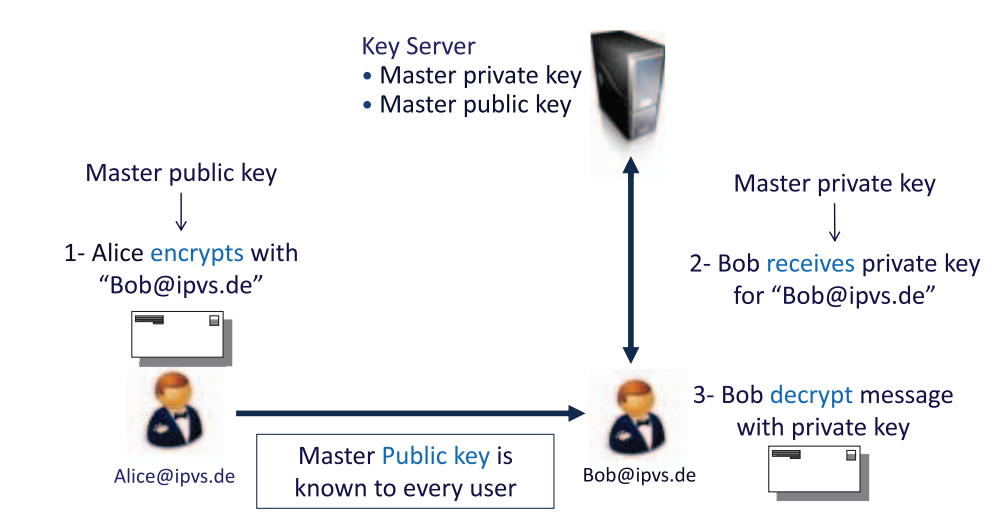
\includegraphics[scale=0.45]{ide.png}
%\caption{\label{fig1 Identity-based encryption[1]}
\caption{\label{a}Identity-based encryption [1]}
%\label{}
\end{figure}

Although identity-based encryption has been proposed
some time ago, only recently pairing-based cryptography
(PBC) has laid the foundation of practical implementation
of identity-based encryption. Pairing-based cryptography
establishes a mapping between two cryptographic groups
by means of bilinear maps. This allows the reduction of one
problem in one group to a different usually easier problem
in another group. This system utilize bilinear maps for establishing
the basic security mechanisms in the pub/sub system and,
therefore, introduce here the main properties.Let  $\mathbb{G}_1 $ and$\mathbb{G}_2 $ be cyclic group of order q,where q is some large prime.A bilinear map is a function $\hat{e}:\mathbb{G}_1  X \mathbb{G}_1\rightarrow \mathbb{G}_1$ that  associates a pair of elements from $\mathbb{G}_1$  to elements in $\mathbb{G}_2$
\pagebreak
\chapter{APPROACH OVERVIEW}
\label{chap:propos}
Publishers and subscribers interact with
a key server. They provide credentials to the key server and
in turn receive keys which fit the expressed capabilities in
the credentials. Subsequently, those keys can be used to
encrypt, decrypt, and sign relevant messages in the content-based pub/sub system, i.e., the credential becomes authorized by the key server. A credential consists of two parts:
1) a binary string which describes the capability of a peer in
publishing and receiving events, and 2) a proof of its
identity. The latter is used for authentication against the key
server and verification whether the capabilities match the
identity of the peer. While this can happen in a variety of
ways, for example, relying on challenge response, hardware
support, and so on, we pay attention mainly at expressing
the capabilities of a credential, i.e., how subscribers and
publishers can create a credential. This process needs to
account for the many possibilities to partition the set of
events expressed by an advertisement or subscription and
exploits overlaps in subscriptions and publications. 

The keys assigned to publishers and subscribers, and the
cipher texts, are labeled with credentials. In particular, the
identity-based encryption ensures that a particular key can
decrypt a particular cipher text only if there is a match
between the credentials of the cipher text and the key.
Publishers and subscribers maintain separate private keys
for each authorized credential.

The public keys are generated by a string concatenation
of a credential, an epoch for key revocation, a symbol $\epsilon\{ SUB, PUB\}$ distinguishing publishers from subscribers. The public keys can be easily generated by any peer
without contacting the key server or other peers in the
system. Similarly, encryption of events and their verification using public keys do not require any interaction.

Due to the loose coupling between publishers and
subscribers, a publisher does not know the set of relevant
subscribers in the system. Therefore, a published event is
encrypted with the public key of all possible credentials,
which authorizes a subscriber to successfully decrypt the
event. The cipher texts of the encrypted event are then signed
with the private key of the publisher, as shown in Fig.4.1.
The overlay network is maintained according to the
containment relationship between the subscriptions. Subscribers with coarser subscriptions are placed near the root
and forward events to the subscribers with less coarser
subscriptions. To maintain such a topology, each subscriber
should
 know the subscription of its parent and child peers.
When a new subscriber arrives, it sends the connection
request (CR) along with its subscription to a random peer
in the overlay network. The connection request is for-warded by possibly many peers in the overlay network
before it reaches the right peer to connect. Each forwarding
peer matches the subscription in the request with the
subscription of its parent and child peers to decide the
forwarding direction. Maintaining a relationship between
subscriptions clearly contradicts subscription confidentiality. Therefore,system proposes an approach to ensure a weaker
notion of subscription confidentiality.
\begin{figure}[htp]
\centering
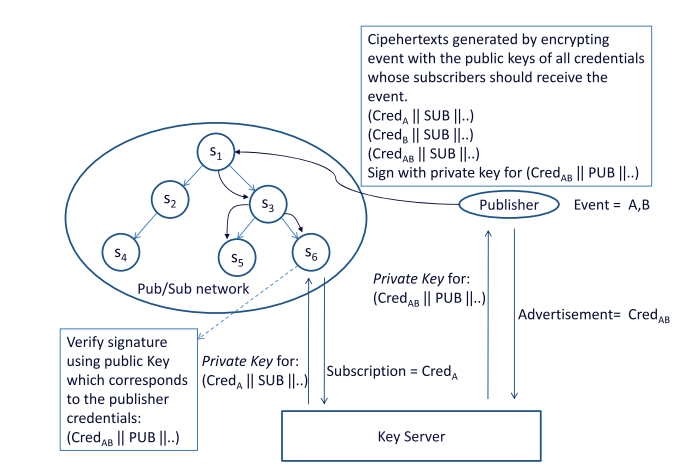
\includegraphics[scale=0.45]{app.png}
%\caption{2.Approach overview[1]}
\caption{\label{a} Approach overview [1]}
%\label{}
\end{figure}
}

\pagebreak
\chapter{CREATION OF CREDENTIALS}
\label{chap:fut}In the following,  first describe the creation of
credentials for numeric and string attributes.
\section{Numeric Attributes}
The event space, composed of d distinct numeric attributes,
can be geometrically modeled as a d-dimensional space
such that each attribute represents a dimension in the space.
With the spatial indexing approach, the event space is
hierarchically decomposed into regular subspaces, which
serve as enclosing approximation for the subscriptions,
advertisements, and events. The decomposition procedure
divides the domain of one dimension after the other and
recursively starts over in the created subspaces. Fig.5.1
visualizes the advancing decomposition with the aid of a
binary tree.

Subspace are identified by a bit string of "0" and "1"s. A
subspace represented by $dz_1$ is covered by the subspace
represented by $dz_2$,if $dz_2$ is a prefix of $dz_1$. Subscription or
advertisement of a peer can be composed of several
subspaces. A credential is assigned for each of the mapped
subspace.To deliver the encrypted event, a
cipher text must be generated for each subspace that
encloses the event so that the peer whose subscription
mapped to any of these subspaces should be able to
successfully decrypt the event.

\begin{figure}[htp]
\centering
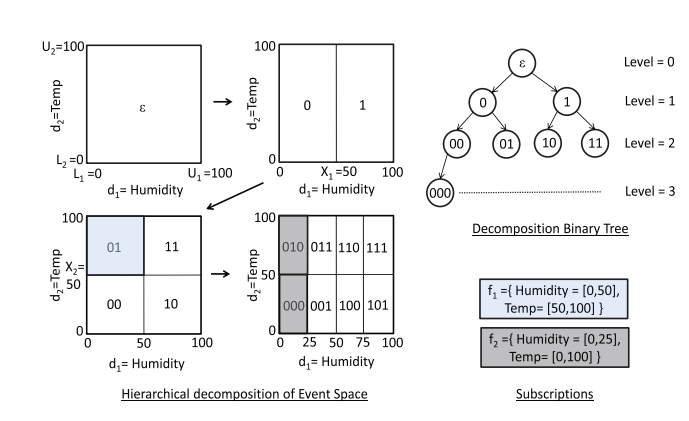
\includegraphics[scale=0.45]{numeric.png}
\caption{\label{a}Numeric Attribute[1]}
%\label{}
%\caption{\label{a} Multisource VoD in CR wireless mesh networks [1]}
\end{figure}
}
Credentials for more expressive string operations such as
prefix matching can be generated using a trie. Each node in
the trie is labeled with a string, which serves as a common
prefix to all its descendants, as shown in Fig.5.2. Each peer is
assigned a single credential, which is same as its subscription or advertisement. Events correspond to the leaf nodes
of the trie. To deliver an encrypted event, a cipher text must
be generated with the label of each node in the path from
the leaf to the root of the trie, so that a peer whose
subscription matches any of the labels should be able to
successfully decrypt the event.
\begin{figure}[htp]
\centering
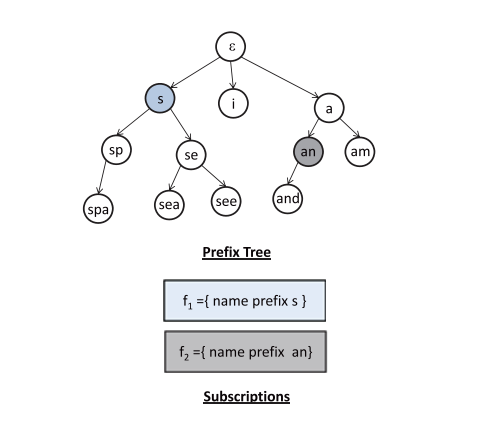
\includegraphics[scale=0.45]{string.png}
\caption{\label{a}Prefix matching[1]}
%\label{}
\end{figure}
}

\pagebreak
\clearpage
\chapter{PUBLISHER/SUBSCRIBER AUTHENTICATION AND EVENT CONFIDENTIALITY}
The security methods describe here are built
upon cipher text-policy attribute-based encryption (in short
CP-ABE) scheme. In particular, our modifications 1) allow publishers to sign and
encrypt events at the same time by using the idea of the
identity-based signcryption ,2) enable efficient routing of encrypted events (from
publishers to subscribers) by using the idea of searchable
encryption and 3) allow
subscribers to verify the signatures associated with all the
attributes (of an event) simultaneously.\
\section{Security Parameters and Initialization}
Let  $\mathbb{G}_1 $ and$\mathbb{G}_2 $ be bilinear group of order q,where q is some large prime.Consider a  bilinear map $\hat{e}:\mathbb{G}_1  X \mathbb{G}_1\rightarrow \mathbb{G}_1$ and $\textit{g}$ is a generator in $\mathbb{G}_1$ \
\begin{algorithm}
  \caption{The initialization algorithm}
  \label{alg2}
  \begin{algorithmic}[1]
  \State{Chooses $\propto,\varphi \in  \mathbb{Z}_q$}
   \State{Computes $g_1=g^{\propto}$ and $h=g^{\varphi}$}
  \State {Chooses $g_2 ,u^{'},m^{'} \in \mathbb{G}_1$ and}
  \state {Selects vectors $\vec{u}=(u_i)$ and $\vec{m}=(m_i)$ of length $n_u$ and $n_m$ respectively , with every element chosen uniformly at random from $\mathbb{G}_1$} 
  
\end{algorithmic}
\end{algorithm}
The master public key ${MP}_u$is known to every peer in the system and is used for encryption and signature
verification. The Master Private key ${MP}_r$ is
only known to the key server. The master private key is
used for generating private keys for publishers and
subscribers.
\section{Key Generation for Publishers/Subscribers}
\textbf{Publisher keys}:Before starting to publish events, a publisher contacts the key server along with the credentials for each
attribute in its advertisement. If the publisher is allowed to
publish events according to its credentials, the key server
will generate separate private keys for each credential. Let
${Cred}_{i,j}$ denote the credential with label j for
 the attribute $A_i$.The public key of a publisher p for credential ${Cred}_{i,j}$
is generated as
\begin{equation}
\label{eq-quad}
Pu_{i,j}^p=(Cred_{i,j}||A_i||PUB||Epoch)
\end{equation}

The key server will generate the corresponding private keys
as follows: For each credential $Cred_{i,j}$ and a publisher p, let$v_p =H_1( Pu_{i,j}^p)$ be a bit string of length $n_u$ and let $v_p[k]$
denote the Kth bit. Let$\Gamma _{i,j} \subseteq{1,2,...n_u}$ be set of all k for $v_p[k]=1$. The key server chooses $\gamma_{i,j}\in \mathbb{Z}_q$ at
random and computes
\begin{equation}
\label{eq-quad}
Pr_{i,j}^p=({g_{2}}^\alpha(u^{'}\prod_{k\in \Gamma _{i,j}}                     u_k)^{\gamma_{i,j}},g^{\gamma_{i,j}})=Pr_{i,j}^p[1],Pr_{i,j}^p[2]
\end{equation}

\noindent
\textbf{Subscriber keys};Similarly, to receive events matching its
subscription, a subscriber should contact the key server and
receive the private keys for the credentials associated with
each attribute $A_i$. In case of subscribers, the public key for a
credential $Cred_{i,j}$ is given as 
\begin{equation}
\label{eq-quad}
Pu_{i,j}^s=(Cred_{i,j}||A_i||SUB||Epoch)
\end{equation}
The private keys for subscriber is
\begin{equation}
\label{eq-quad}
Pr_{i,j}^s=({g_{2}}^{\gamma_s}(u^{'}\prod_{k\in \Gamma _{i,j}} u_k)^{\gamma_{i,j}},g^{\gamma_{i,j}},H_3(u^{'}\prod_{k\in \Gamma _{i,j}} u_k)^{\varphi})=(Pr_{i,j}^s[1],Pr_{i,j}^s[2],Pr_{i,j}^s[3])
\end{equation}
Furthermore, a credential independent key  $Pr_{i,j}^s[4]={g_2}^{\frac{\gamma_s+\alpha}{\varphi}}$
generated. This key along with$ \gamma_s$ is
needed to bind the keys/credentials of a subscription
together.
\section{Publishing and Receiving  Events}
\textbf{Encryption}:When a publisher wants to publish an event
message M, it chooses $b_i \in \mathbb{Z}_q$ at random for each attribute
$A_i$ of the event. These random values ensure that only the subscribers who have matching
credentials for each of the attributes should be able to
decrypt the event. Furthermore, the publisher generates a
fixed-length random key SK for each event.

\noindent
\textbf{Decryption}:On receiving the cipher texts, a subscriber tries to
decrypt them using its private keys. The cipher texts for each
attribute are strictly ordered according to the containment
relation between their associated credentials; therefore, a
subscriber only tries to decrypt the cipher text whose
position coincides with the position of its
 credential in the containment hierarchy of the corresponding attribute. The
position of a credential can be easily determined by
calculating its length.
\pagebreak
\clearpage
\chapter{SUBSCRIPTION CONFIDENTIALITY}
This section addresses to achieve subscription confidentiality in a broker-less pub/sub system.
\section{Publish/Subscribe Overlay}
The pub/sub overlay is a virtual forest of logical trees,
where each tree is associated with an attribute  A subscriber joins the trees corresponding to the attributes of
its subscription. Similarly, a publisher sends an event on all
the trees associated with the attributes in the event.


Within each attribute tree, subscribers are connected
according to the containment relationship between their
credentials associated with the attribute. The subscribers
with coarser credentials (e.g., the ones mapped to coarser
subspaces in case of numeric attributes) are placed near the
root of the tree and forward events to the subscribers with
finer credentials. A subscriber with more than one
credentials can be handled by running multiple virtual
peers on a single physical node, each virtual peer maintaining its own set of tree links, as shown in Fig.7.1. To
connect to an attribute tree, a newly arriving subscriber $s_n$
sends the connection request along with its credential to a
random peer $s_r$in the tree. The peer $s_r$ compares the request
credential with its own; if the peer’s credential covers the
request credential and the peer can accommodate more
children, it accepts the connection. Otherwise, the connection request is forwarded to all the children with covering
credentials and the parent peer with the exception of the
peer from which it was received. In this way, the connection
request is forwarded by many peers in the tree before it
reaches the suitable peer with covering credential and
available connection, as shown in Fig.7.1.
\newpage
\vspace*{10pt}
 \begin{figure}[htp]
\centering
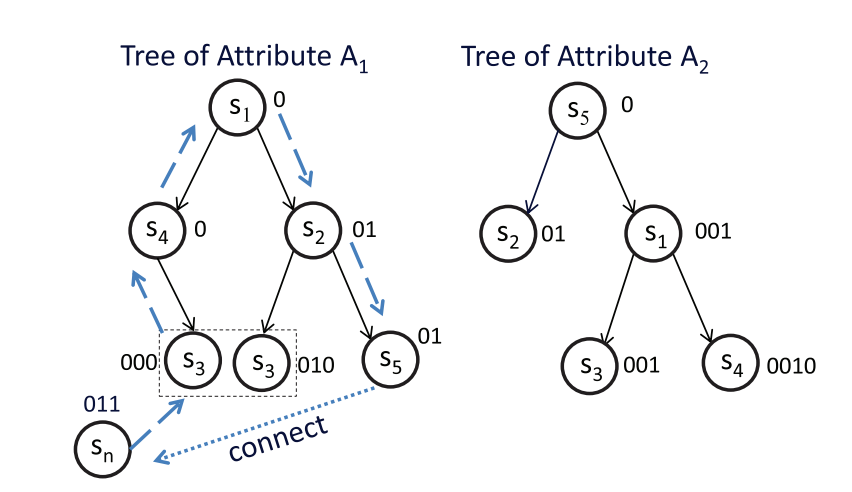
\includegraphics[scale=0.45]{pubsub.png}
\caption{\label{a}Publish/Subscribe System with two numeric attributes[1] }
%\label{}
\end{figure}

\section{Weak Subscription Confidentiality}
It is infeasible to provide strong subscription confidentiality in a broker-less pub/sub system because the maintenance of the overlay topology requires each peer to know
the subscription of its parent as well as its children. To
address this issue, a weaker notion of subscription
confidentiality is required.
\textbf{Definition}:Let $s_1$ and $s_2$ denote two subscribers in a pub/sub
system which both possess credentials for an attribute$A_i$.Weak subscription confidentiality ensures that at most the
following information can be inferred about the credentials of
the subscribers:
:\\
1. The credential of $s_1$ is either coarser or equal to the
credentials of $s_2$.\\
2. The credential of $s_1$ is either finer or equal to the
credentials of $s_2$.\\
3. The credentials of $s_1$ and $s_2$ are not in any containment
relationship.
\section{Secure Overlay Maintenance}
In the following section ,the system propose a secure protocol to maintain
the desired pub/sub overlay topology without violating the
weak subscription confidentiality. For simplicity and with-out loss of generality, here we discuss the overlay maintenance with respect to  a single tree associated with a numeric attribute
$A_i$ and each of the subscribers owns a single credential.


The secure overlay maintenance protocol is based on the
idea that in the tree, subscribers are always connected
according to the containment relationship between their
credentials.A new subscriber s generates a random key SW and
encrypts it with the public key  $Pu_{i,j}^s$ for all credentials that
cover its own credential.The generated cipher texts are
added to a connection request (CR) and the request is
forwarded to a random peer in the tree. A connection is
established if the peer can decrypt any of the cipher texts
using its private keys.

A different random key SW is used for the generation of
each cipher text to avoid any information leak to the peer
who has successfully decrypted one of the cipher texts and,
thus, has recovered the random key SW. Finally, to avoid
an attacker to generate arbitrary connection request
messages and try to discover the credential of other peers
in the system, the connection request is signed by the key
server.\\
\begin{algorithm}
  \caption{Secure Overlay Maintenance Protocol}
  \label{alg3}
  \begin{algorithmic}[1]
  \State{\textbf{upon event} Receive(CR of $s_{new}$ from $s_p$)\textbf{do}}
   \State  $~$ \hspace{0.25cm} \textbf{if}  \textit{decrypt-request(CR)==SUCCESS } \textbf{then}
  \State $~$ $~$ $~$\hspace{0.45cm} \textbf{if}  \textit{degree($s_q$)} == available \textbf{then}   //can have child peers
 \State $~$ $~$ $~$ $~$\hspace{0.6cm} connect to the $s_{new}$
 \State $~$ $~$ $~$\hspace{0.45cm} \textbf{else}
 \State $~$ $~$ $~$ $~$\hspace{0.6cm}forward CR to\textit {child peers and parent}-$s_p$
 \State $~$\hspace{0.25cm} \textbf{if}  \textit{decrypt-request(CR)==FAIL} \textbf{then}
\State$~$ $~$ $~$\hspace{0.45cm} \textbf{if} $s_p$==parent \textbf{then}
 \State $~$ $~$ $~$ $~$\hspace{0.6cm}Try to swap by sending its own CR to the $s_{new}$
\State $~$ $~$ $~$\hspace{0.35cm} \textbf{else}
\State $~$ $~$ $~$ $~$\hspace{0.55cm} forward to parent
 
\end{algorithmic}
\end{algorithm}
\section{ Secure Event Dissemination}
To publish an event, a publisher forwards the cipher texts of
each attribute to the root of the corresponding attribute tree.
All the cipher texts of an event are labeled with a unique
value such as sequence number of the event.In this section, two strategies are proposed  to
route events (from publishers to the relevant subscribers) in
the pub/sub overlay network without violating the weak
subscription confidentiality\\
\textbf{One-hop flooding (OHF)}:In one-hop flooding, a parent
assumes that the children have the same credentials as its
own and forward each successfully decrypted event to all of
them. In turn, the children forward each event which was
successfully decrypted to all of their children and so on.Moreover a child may have finer credentials than its parent and
may receive false positives.

\textbf{Multicredential routing (MCR)}:MCR strategy targets
reduction in false positives by enabling parents to forward
only those event on each attribute tree that match the
credential of their children.  More precisely,
the decision (DEC) to forward cipher texts associated with
an attribute$A_i$ to the child can be described as
\begin{equation}
\label{eq-quad}
DEC=
\begin{cases}
 \begin{array}{lcl}
$$forward, if $$ H_4(\hat{e}(Pr_{i,{\tau}_i}^s[3],{CT}_i)) =CT'_{i,{\tau}_i}\\
$$drop , otherwise$$
 \end{array}
 \end{cases}
\end{equation}

Although the actual credentials of children are hidden from
the parent peers by the use of $Pr_{i,j}^s[3]$ keys. Nevertheless, the
hidden credentials are not adequate to
ensure weak subscription confidentiality. This is because a
parent decrypts every event which it forward to its children
and, therefore, can eventually discover their credentials, for
example, by maintaining histories of the events forwarded
to each child.

To preserve weak subscription confidentiality, subscribers divide the original credential(s) for each attribute of
their subscriptions into a number of fine granular credentials and $Pr_{i,j}^s[3]$ key for each (fine granular) credential is
forwarded to a separate parent in the corresponding
attribute tree.

To ensure that a
subscriber always connects to a distinct parent for each of
its credentials, techniques such as broadcast revocation can
be used . It is also important to mention that the
subscribers cannot generate $Pr_{i,j}^s[3]$ keys for the fine
granular credentials obtained as a result of dividing the
original credential(s) and, therefore, should contact the key
server for the creation of $Pr_{i,j}^s[3]$ keys. This step can be
performed at the same time when a new subscriber
authorizes itself to the key server.
\chapter{PERFORMANCE EVALUATION}
This section  evaluates 
performance and scalability of the proposed pub/sub
system only with respect to the security mechanisms and
omit other aspects. In particular, we evaluate the performance of our system with respect to the overlay construction time
and the event dissemination delays.\\
 \begin{figure}[htp]
\centering
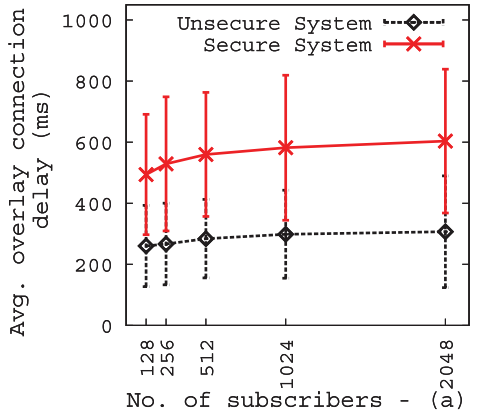
\includegraphics[scale=0.6]{perf1.png}
\caption{\label{a}Performance Evaluations [1]}
%\label{}
\end{figure}

In Fig.8.1, we measure the average delay experienced by
each subscriber to connect to a suitable position in an
attribute tree. Delay is measured from the time a subscriber
sends connection request message to a random peer in the
tree till the time the connection is actually established. The
evaluations are performed only for a single attribute tree.
Fig.8.1 shows that the average connection time (delay)
increases with the number of peers in the system because of
the increase in the height of the attribute tree (each new hop
increases the network delay as well as time to apply
security methods). Furthermore, Fig. 8.1 shows that there is an overhead of approximately 230-300 ms due to security
mechanisms.


\begin{figure}[htp]
\centering
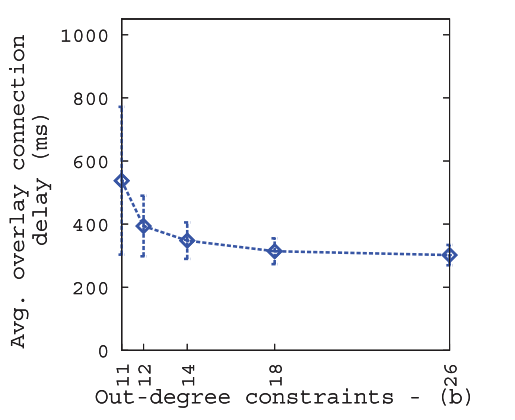
\includegraphics[scale=0.6]{perf2.png}
\caption{\label{a}Performance Evaluations[1] }
%\label{}
\end{figure}
Fig. 8.2 shows that for a fixed set of peers, the average delay
experienced by subscribers decreases significantly with the
increase in out-degree mainly because the resultant dissemination tree is fat (i.e., tree with smaller height). For the
similar reason, Fig. 8.1 reports that average connection time
(delay) increases very slightly with the number of peers.
The increase in the average connection delay is small
because the overall out-degree also increases with the
number of peers, resulting in only a small increase in the
height of the tree
\begin{figure}[htp]
\centering
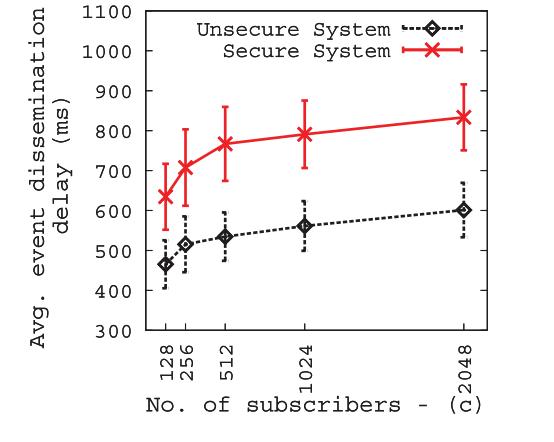
\includegraphics[scale=0.6]{perf3.png}
\caption{\label{a}Performance Evaluations[1] }
%\label{}
\end{figure}

Fig. 8.3 measures the average time needed by the event
to be disseminated to all the relevant subscribers in the
system. For each subscriber, the time is measured from the
dissemination of the event by the publisher till it is
successfully decrypted and verified by the subscriber. For
the experiment, 160 publishers are introduced in the
system and each published 10 events. Fig. 8.3 shows that
the average time to disseminate an event increases with
the number of peers in the system because of the increase
in number of the relevant subscribers as well as the height
of the dissemination tree. Similar to the previous results,
there is an overhead of approximately 150-250 ms due to
security mechanisms.

\chapter{CONCLUSION AND FUTURE WORK}
This system proposed a new approach to provide
authentication and confidentiality in a broker-less content-based pub/sub system. The approach is highly scalable in
terms of number of subscribers and publishers in the
system and the number of keys maintained by them. In
particular, we have developed mechanisms to assign
credentials to publishers and subscribers according to their
subscriptions and advertisements. Private keys assigned to
publishers and subscribers, and the cipher texts are labeled
with credentials.It from identity-based encryption 1) to ensure that a particular subscriber
can decrypt an event only if there is a match between the
credentials associated with the event and its private keys
and 2) to allow subscribers to verify the authenticity of
received events. Furthermore, we developed a secure
overlay maintenance protocol and proposed two event
dissemination strategies to preserve the weak subscription
confidentiality in the presence of semantic clustering of
subscribers.


Certificate less cryptography is  a variant of identity based cryptography that prevent the key escrow problem.In Identity Based   ,dependence on PKG who use master key to generate private key introduces key escrow.And also compromise of PKG master key could be disastrous in  proposed system.So Certificate less cryptography is an efficient method to solve the problems associated with   Identity Based Encryption which will be addressed in future.
\pagestyle{empty}
\begin{singlespace}
  %\bibliography{refs}
  \begin{thebibliography}{1}
\bibitem{}
Muhammad Adnan Tariq, Boris Koldehofe, and Kurt Rothermel,\textit{"Securing Broker-Less Publish/Subscribe Systems Using Identity-Based Encryption"},IEEE Transactions on parallel and distributed systems,February 2014

\bibitem{}
C. Raiciu and D.S. Rosenblum, \textit{"Enabling Confidentiality in
Content-Based Publish/Subscribe Infrastructures,"}Proc. IEEE
Second CreatNet Int’l Conf. Security and Privacy in Comm. Networks
(SecureComm),2006.
\bibitem{}
M. Srivatsa, L. Liu, and A. Iyengar, \textit{"EventGuard: A System
Architecture for Securing Publish-Subscribe Networks"}ACM
Trans. Computer Systems,vol. 29, article 10, 2011.

\bibitem{}
A. Shikfa, M. O¨
nen, and R. Molva, \textit{"Privacy-Preserving Content-Based Publish/Subscribe Networks,"}Proc. Emerging Challenges for
Security, Privacy and Trust,2009.
\bibitem{}
RobertoBaldoni, Mariangela Contenti, and Antonino Virgillito, \textit{" The Evolution of Publish/Subscribe
Communication Systems,"} 

\bibitem{}
Ying Liu Beth Plale
,,\textit{ "Survey of Publish Subscribe Event Systems,"}
\bibitem{}
E. Anceaume, M. Gradinariu, A.K. Datta, G. Simon, and A.
Virgillito, \textit{"A Semantic Overlay for Self- Peer-to-Peer Publish/
Subscribe,"} Proc. 26t
\bibitem{}
J. Bacon, D.M. Eyers, J. Singh, and P.R. Pietzuch, \textit{"Access Control
in Publish/Subscribe Systems,"} Proc. Second ACM Int’l Conf.
Distributed Event-Based Systems (DEBS),2008
\bibitem{}
W.C. Barker and E.B. Barker, \textit{"SP 800-67 Rev. 1. Recommendation
for the Triple Data Encryption Algorithm (TDEA) Block Cipher,"}
technical report, Nat’l Inst. of Standards & Technology, 2012
\bibitem{}
J. Bethencourt, A. Sahai, and B. Waters, \textit{"Ciphertext-Policy
Attribute-Based Encryption,"}Proc. IEEE Symp. Security and
Privacy,2007

\end{thebibliography}
\end{singlespace}


  
\end{document}

